\chapter{Cause-Effect Pair Extraction}\label{ch:cause-effect-extraction}
This chapter will provide a methodology to extract multiple \ac{CEP}s from a sentence, by using dependency patterns and a novel phrase extraction algorithm.


\section{Natural Language Processing}\label{sec:natural-language-processing}

\begin{figure}
    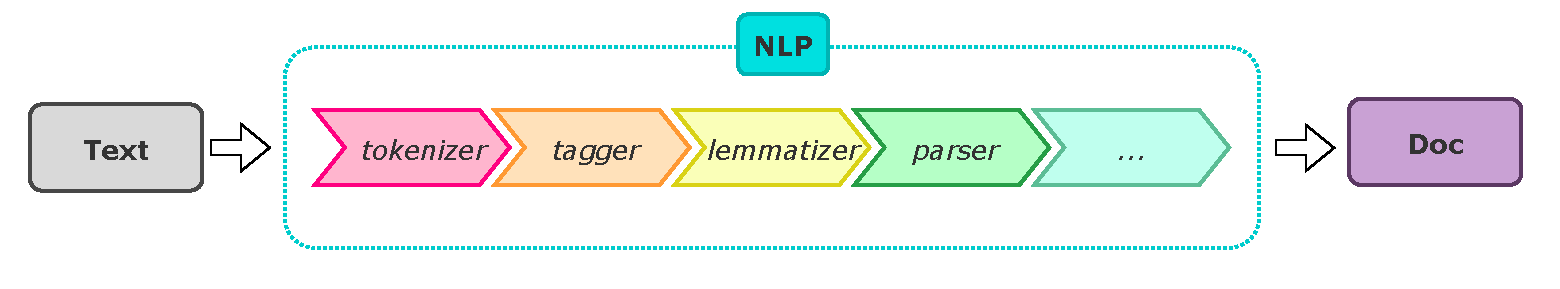
\includegraphics[width=\textwidth]{figures/cause_effect_extraction/spacy_pipeline}
    \caption{NLP Pipeline}\label{fig:spacy-pipeline}
\end{figure}

The first step of our extraction algorithm takes a text and pass it through a \ac{NLP} pipeline.
Fortunate, several NLP libraries such as spaCy utilizes such pipelines with pretrained models to add linguistic features to the text.
In \autoref{fig:spacy-pipeline} we can see the simplified pipeline for the \qq{en\_core\_web\_lg} model\footnote{\url{https://spacy.io/models/en\#en_core_web_lg}} from the spaCy library.
Such pipeline can contain several of different layers and implementation details.
Our approach to \ac{CEP}s is based on dependency patterns.
Thus, the pipeline needs to have a tokenizer, tagger, lemmatizer and parser.

\subsection{Tokenizer}\label{subsec:tokenizer}
The tokenizer splits the text into meaningful segments, called tokens.
These tokens could be words, punctuations, combinations of abbreviations or other segments.
For example the word \qq{don’t} should be divided into two tokens whereas a word like \qq{v1.0} should be remains at one token.
There are several implementations of such tokenizer, we used the built-in tokenizer from spaCy which first splits the raw text based on whitespace characters.
Next, the algorithm loops over the substrings and tries to split them into more granular tokens based on different rules, such as prefix, suffix, punctuation and more.
The tokens are the foundation for the following pipeline.

\subsection{Tagger}\label{subsec:part-of-speech-tagging}
The first label added to the tokens is the \ac{POS}\footnote{\url{https://universaldependencies.org/u/pos/}} label.
This tag can be divided into three groups.
The first group contains open class words such as adjective (ADJ), noun (NOUN), proper noun (PROPN) or verb (VERB).
The second group are closed class words such as determiner (DET) or pronoun (PRON).
The last group contains the other tags such as punctuation (PUNCT).

\subsection{Lemmatizer}\label{subsec:lemmatizer}
The next component is the lemmatizer which groups different inflected forms into a single word.
For example, the words \qq{works}, \qq{worked} or \qq{working} would have all the same lemma \qq{work}.
Another advantage of a lemmatizer is that it also does the morphological analysis of words.
Thus, it detects \qq{good} as a lemma for the word \qq{better}, which is especially useful if we want to compare different tokens with each other.

\subsection{Parser}\label{subsec:dependency}
The last step is the dependency parser which adds the \ac{DEP}\footnote{\url{https://downloads.cs.stanford.edu/nlp/software/dependencies_manual.pdf}} tag to a token.
This preprocessing step connects different tokens with each other, which allows us to represent the sentence in a dependency tree and apply dependency patterns to the sentence.
For example, the \qq{nsubj} tag defines a syntactic subject of a clause.
In \autoref{sec:dependency-matching} we will see the needed \ac{DEP} tags to define the dependency patterns.


\section{Dependency Matching Patterns}\label{sec:dependency-matching}
After pre-processing the sentence by passing it through an \ac{NLP} pipeline, we want to find the root tokens for the \ac{CEP}.
In \cite{doan2019extracting, sorgente2013automatic}, the authors provided dependency patterns to identify \ac{CEP}s with a single word.
For example, if we look at the sentence \qq{A GPS fault causes a crash.}, these patterns find \qq{fault} => \qq{crash} as a \ac{CEP}.
We implement these patterns using the DependencyMatcher\footnote{\url{https://spacy.io/usage/rule-based-matching\#dependencymatcher}} from spaCy, which utilizes Semgrex operators on a dependency tree to match patterns.
In \autoref{fig:pattern-simple}, \autoref{fig:pattern-phrasal} and \autoref{fig:pattern-passive} on the left side are example patterns that can be implemented with the DependencyMatcher.
These patterns consist of nodes that are connected over Semgrex operators.
For example, the node \qq{A} and \qq{B} defines a pattern with the \qq{>} Semgrex operator, which looks like \qq{A > B}.
The pattern matches when in the dependency tree the node \qq{A}, the immediate head of \qq{B} is.
We can add attributes to the nodes that define additional rules that the node needs to fulfill.
For example, we could specify a lemma representation of a word that we want to match or a specific \ac{POS} tag that needs to be fulfilled.
Furthermore, these patterns have one anchor node, which is equivalent to a root in a tree, which is the starting point for the DependencyMatcher.
We use this anchor node to find explicit causal mentions based on a list of low ambiguity and high frequency causation verbs provided by \cite{girju2002text}.
The most common causal identifiers are \qq{cause}, \qq{lead}, \qq{generate} and \qq{trigger}.
Furthermore, we used a verb list consisting of 26\footnote{cause, generate, trigger, induce, produce, effect, provoke, arouse, elicit, lead, derive, associate, relate, link, stem, iginate, result, entail, commence, spark, evoke, implicate, activate, actuate, kindle, stimulate, unleash, effectuate} verbs.
We are now building our anchor node by specifying the lemmatized verb list as additional rule.
Thus, we are able to find different variations of the verb \qq{cause} like \qq{causes} or \qq{caused}.
Based on this anchor node we specify outgoing dependency nodes which are connected to the root token for the cause and the effect in the \ac{CEP}.

\subsection{Simple Causative Verbs}\label{subsec:simple-causative-verbs-pattern}
\begin{figure}
    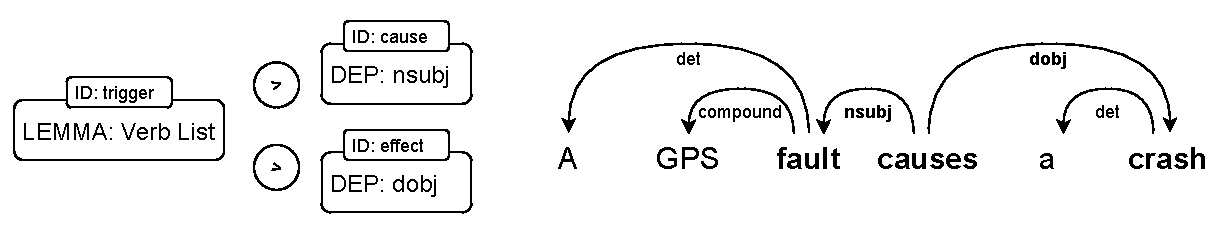
\includegraphics[width=\textwidth]{figures/cause_effect_extraction/simple_pattern}
    \caption{Simple Causative Verbs Pattern}\label{fig:pattern-simple}
\end{figure}
The pattern has as anchor having the meaning of a simple \qq{causal action} such as \qq{cause}, \qq{generate}, or \qq{trigger}.
In this pattern, the cause is the subject of that simple verb, and the effect is the verb's object, which can be seen on the left side of the \autoref{fig:pattern-simple}.
Furthermore, we can see on the right side of \autoref{fig:pattern-simple} an example sentence that is covered by this pattern.
By comparing the sentence with the pattern, we see how dependency matching works.
First, the causal anchor is selected like \qq{causes} which is then be used to find the other tokens that match with the described pattern like \qq{fault} and \qq{crash}
The DependencyMatcher then provides the tokens that match with the pattern, thus  \qq{causes} \qq{fault} and \qq{crash}.
Finally, we specified an ID for each node in the pattern to distinguish the tokens.

\subsection{Phrasal Verbs}\label{subsec:phrasal-verbs-pattern}
\begin{figure}
    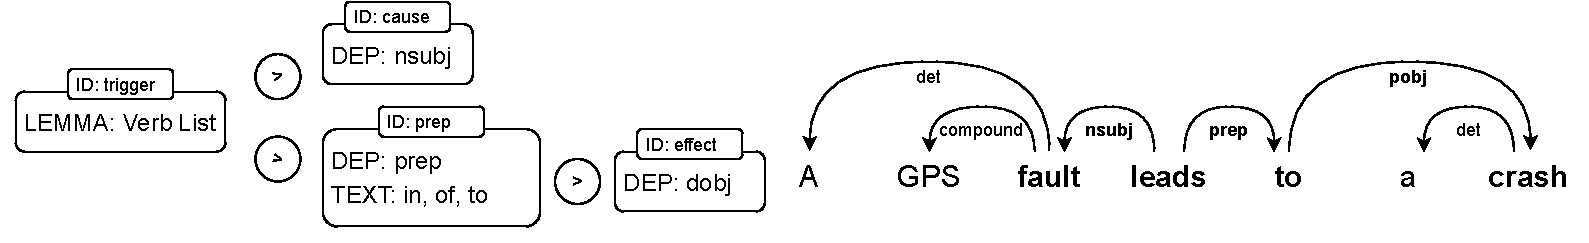
\includegraphics[width=\textwidth]{figures/cause_effect_extraction/phrasal_pattern}
    \caption{Phrasal Verbs Pattern}\label{fig:pattern-phrasal}
\end{figure}
This pattern uses a phrase consisting of a causal verb followed by a preposition like \qq{in}, \qq{of} or \qq{to,} e.g. \qq{lead to} to identify an explicit causal mention.
We then follow the \qq{nsubj} \ac{DEP} from the verb to find the cause and the \qq{pobj} \ac{DEP} from the preposition to find the effect.
In \autoref{fig:pattern-phrasal} we can see the resulting pattern as well as an example sentence that matches with the pattern.

\subsection{Passive Causative Verbs}\label{subsec:passive-causative-verbs-pattern}
\begin{figure}
    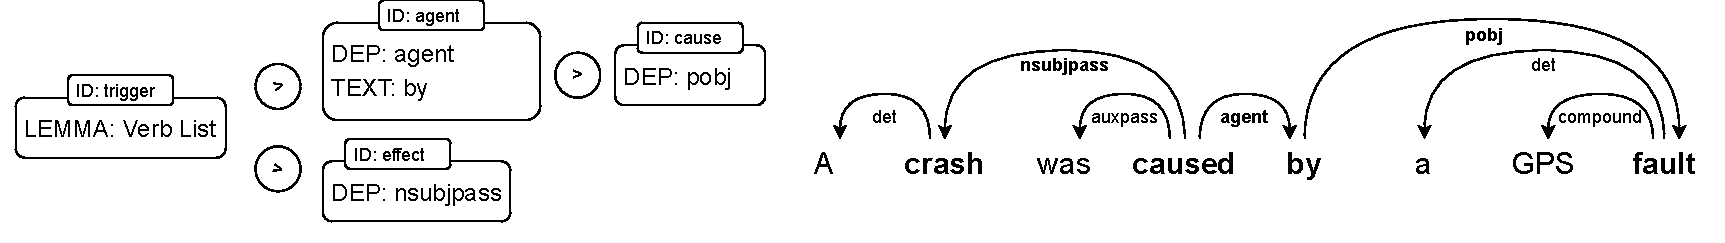
\includegraphics[width=\textwidth]{figures/cause_effect_extraction/passive_pattern}
    \caption{Passive Causative Verbs Pattern}\label{fig:pattern-passive}
\end{figure}
The last pattern we defined is for passive formulations of a sentence.
For example, a user could formulate the same sentence passive like \qq{A crash was caused by a GPS fault} which can be seen in \autoref{fig:pattern-passive}.
Therefore, the pattern uses the preposition \qq{by} that is linked to a verb from the verb list with an \qq{agent} relation.
The \qq{agent} relation is the complement of a passive verb that does the action.
Thus, the cause root is linked with the \qq{pobj} relation to the \qq{by} agent, where \qq{pobj} is the object of a preposition.
The effect is linked with the \qq{nsubjpass} to the causal verb, where \qq{nsubjpass} is a passive nominal subject which is the syntactic subject of a passive clause.
The resulting pattern can be seen in \autoref{fig:pattern-passive}.

\section{Phrase Extraction}\label{sec:phrase-extraction}
With the dependency matching patterns, we are able to identify the root token of the cause and effect.
However, in a sentence from \autoref{fig:pattern-simple} , the resulting \ac{CEP} would be \qq{fault} => \qq{crash} which omits information.
We want to extract phrases that consist of multiple tokens.
Thus, the desired \ac{CEP} looks like \qq{GPS fault} => \qq{crash}.
Furthermore, our current extraction is limited, with only a single CEP extraction on a causal identifier.
We also want to provide a methodology that extracts multiple CEPs that are connected with conjunctions such as \qq{and}, \qq{or}.
In the following, we do not differ between \qq{and}, \qq{or} although in logical rules they have a different meaning.
We decided to do that because in NLP, especially in communication, conjunctions and disjunctions are not applied in a logical way.
Therefore, if a user would say, \qq{A GPS fault, defect motor or empty battery causes a crash} we would extract three \ac{CEP}s \qq{GPS fault} => \qq{crash}, \qq{empty battery} => \qq{crash} and \qq{defect motor} => \qq{crash}.
In the previous example, we saw that the cause from the pairs had no intersecting part and was completely divided by the conjunction.
However, in the sentence \qq{An empty and defect battery causes a crash} the conjunction is between \qq{empty} and \qq{defect} and describes the root token battery.
There are two possible solutions to solve such conjunctions.
The first one is to ignore such conjunctions and extract the whole phrase as one.
We would extract \qq{empty and defect battery} as one phrase.
The second approach is to extract two phrases, \qq{empty battery} and \qq{defect battery}.
We decided to follow the second approach because we want to extract the atomic representation of a \ac{CEP}, which is more suitable to build a causal graph.
We, therefore, want to present a recursive algorithm that is capable of extracting multiple phrases based on a single root token.

\subsection{Algorithm}\label{subsec:algorithm}

\begin{algorithm}
    \algblockdefx{ForEach}{EndForEach}[1]{\textbf{for each} #1 \textbf{then}}{\textbf{end for each}}
    \caption{Phrase Extraction Algorithm}\label{alg:phrase-pseudocode}
    \begin{algorithmic}[1]
        \Require $token$ with dependency links
        \Function{ExtractPhrases}{$token$}

            \If{$token.children$ is empty}
                \State \textbf{return} $[[token]]$
            \EndIf


            \State $phrases \gets []$

            \If{$HasChildrenWithPhraseDependency(token)$}
                \State $children\_phrases \gets []$
                \ForEach{$child \in ChildrenWithPhraseDependency(token)$}
                \State $child\_phrases \gets ExtractPhrases(child)$
                \State $children\_phrases \gets Insert(children\_phrases, child\_phrases)$
                \EndForEach
                \State $combined\_children\_phrases \gets ReduceWithProduct(children\_phrases)$
                \State $token\_phrases \gets InsertAndSortTokenIntoChildrenPhrases(combined\_children\_phrases)$
                \State $phrases  \gets Extend(phrases, token\_phrases)$
            \Else
                \State $phrases  \gets Extend(phrases, [[token]])$
            \EndIf

            \ForEach{$child \in ChildrenWithConjDependency(token)$}
            \State $conj\_phrases \gets ExtractPhrases(child)$
            \State $phrases  \gets Extend(phrases, conj\_phrases)$
            \EndForEach

            \State \textbf{return} $phrases$
        \EndFunction
    \end{algorithmic}
\end{algorithm}

\begin{figure}
    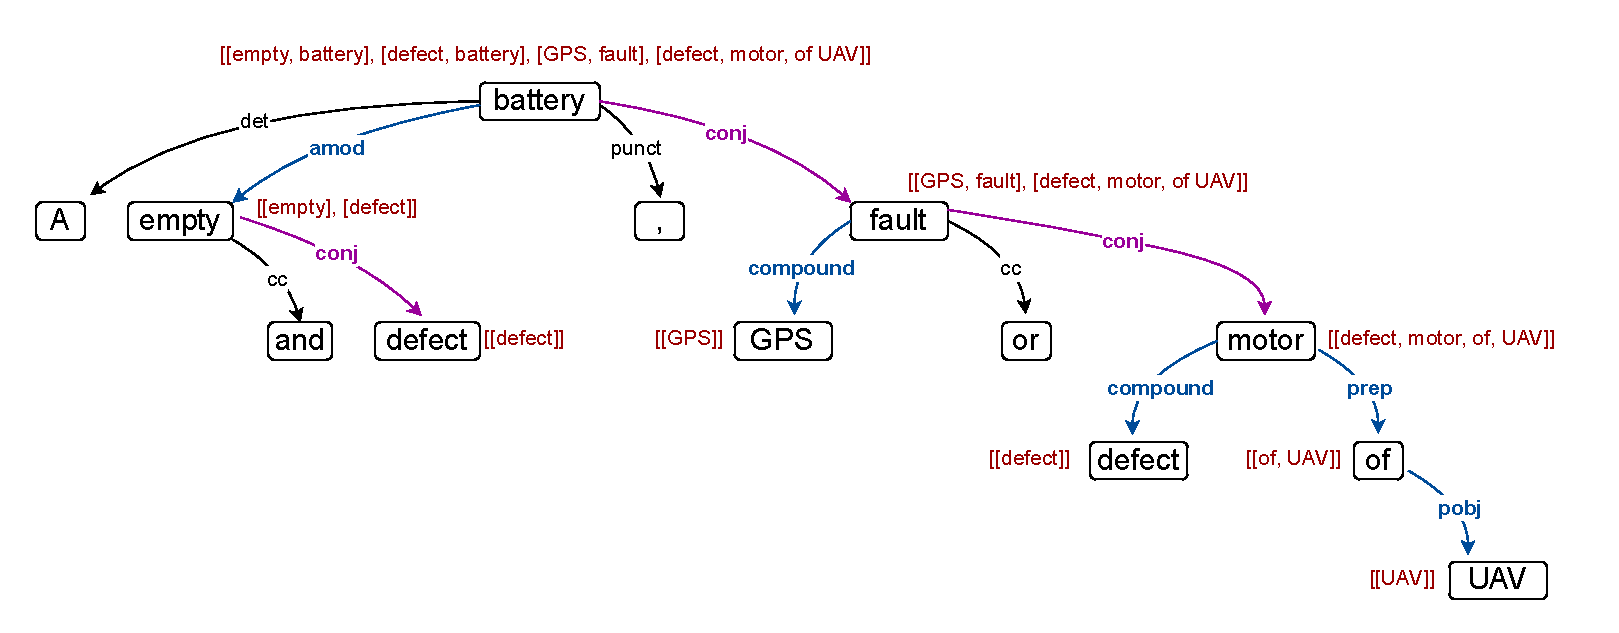
\includegraphics[width=\textwidth]{figures/cause_effect_extraction/phrase_algoirthm_example}
    \caption{Phrase Extraction Algorithm Example}\label{fig:phrase-example}
\end{figure}


In \autoref{alg:phrase-pseudocode} we can see the pseudocode for the phrase extraction algorithm.
The algorithm takes a single token as input and returns multiple phrases.
Thus, it returns a list of lists, where the outer list defines the multiple phrases and the inner lists consist of the tokens in a phrase.
Our recursive algorithm follows the dependency\footnote{Add the dependencies here} links from the input token based on a predefined list of dependencies.
We extend the dependencies from \cite{sharp2016creating} to handle multiple phrases.
In \autoref{fig:phrase-example}, we can see the dependency tree for the sentence \qq{A empty and defect battery, GPS fault or defect motor of UAV causes a crash.}.
This example shows a dependency tree and each interim recursion result at the node level.
The recursion stops at the leaf level of the dependency tree.
We defined the recursion base case by returning a list of a single phrase containing only the leave token (lines 2 to 4).
After defining the base case in the recursion, we need to define how to handle the merge approach.
We have three different cases that we need to handle.
We use the variable phrases (line 5) to store the results from the different cases.
The first case handles all the children linked with a dependency link from the list to the parent node (lines 6 to 15).
We first apply the recursion step to each child token (lines 8 to 11).
We then reduce the different phrases from the tokens into a single list (line 12).
We do so by using the cartesian product between two lists and the results list from the children as input in a higher-order reduce function.
These operations produce multiple phrases that cover all combinations of the phrases from the children.
The last step is to insert the root token into each phrase and sort each phrase based on the occurrence of a token in the sentence (line 13).
We then add the resulting phrases into the phrases variable (line 14).
The second case occurs when the token has no child connected with a dependency from the list line (15 to 17).
We then simply need to add the single token to the phrases list.
An example of why we need this can be seen for the node \qq{empty} in the figure.
Without the previous case, we would not include \qq{empty} in the resulting phrases because there are no children results where we can merge the token into.
The last case (lines 18 to 21) handles the conjunctions dependencies.
Finally, we apply the recursion step for each child that is connected by a conjunction with the token.
With this novel recursive algorithm, we were able to extract four phrases from the example sentence: \qq{empty battery}, \qq{defect battery}, \qq{GPS fault} and \qq{defect motor of UAV}.


\section{Filter Noise Phrases}\label{sec:filter-noise-phrases}
In the previous step, we were able to identify multiple phrases from a single root token.
However, during this expansion, the phrases can contain noise and vague information.
Thus, some phrases need to be filtered or shortened.
We defined that a complete phrase needs to include either a VERB, PROPN, or a NOUN. If a phrase does not contain a token that has such a \ac{POS} tag, we drop the phrase.
We then removed all tokens with the PRON tag such as \qq{I}, \qq{we} or \qq{they}.
Next, we created a list of lemmas e.g., \qq{by}, \qq{any} or \qq{which}, which was manually created by analyzing the extracted phrases.
Finally, we removed the start and end tokens from the phrases based on that list.
Thus, we now have cleaned phrases that can be used to create \ac{CEP}s.


\section{Combine Phrases To Cause-Effect Pairs}\label{sec:combine-the-phrases-to-a-pair}
In \autoref{sec:phrase-extraction} and \autoref{sec:filter-noise-phrases}, we extract and filter phrases based on a single root token.
We use these approaches to find the phrases for the root cause and the root effect in a sentence that we find by applying the patterns from \autoref{sec:dependency-matching}.
The final step is to create \ac{CEP}s from these phrases by combining the phrases with the cartesian product.
In the example sentence from \autoref{sec:phrase-extraction} the root cause was \qq{battery} and the root effect \qq{crash}.
We were able to extract four phrases from \qq{battery} and one phrase from \qq{crash}.
By applying the cartesian product between the phrases we get the \qq{CEP}s: \qq{empty battery} => \qq{crash}, \qq{defect battery} => \qq{crash}, \qq{GPS fault} => \qq{crash} and \qq{defect motor of UAV} => \qq{crash}.
